%%\documentclass[main]{subfiles}

\begin{figure}
    \centering
    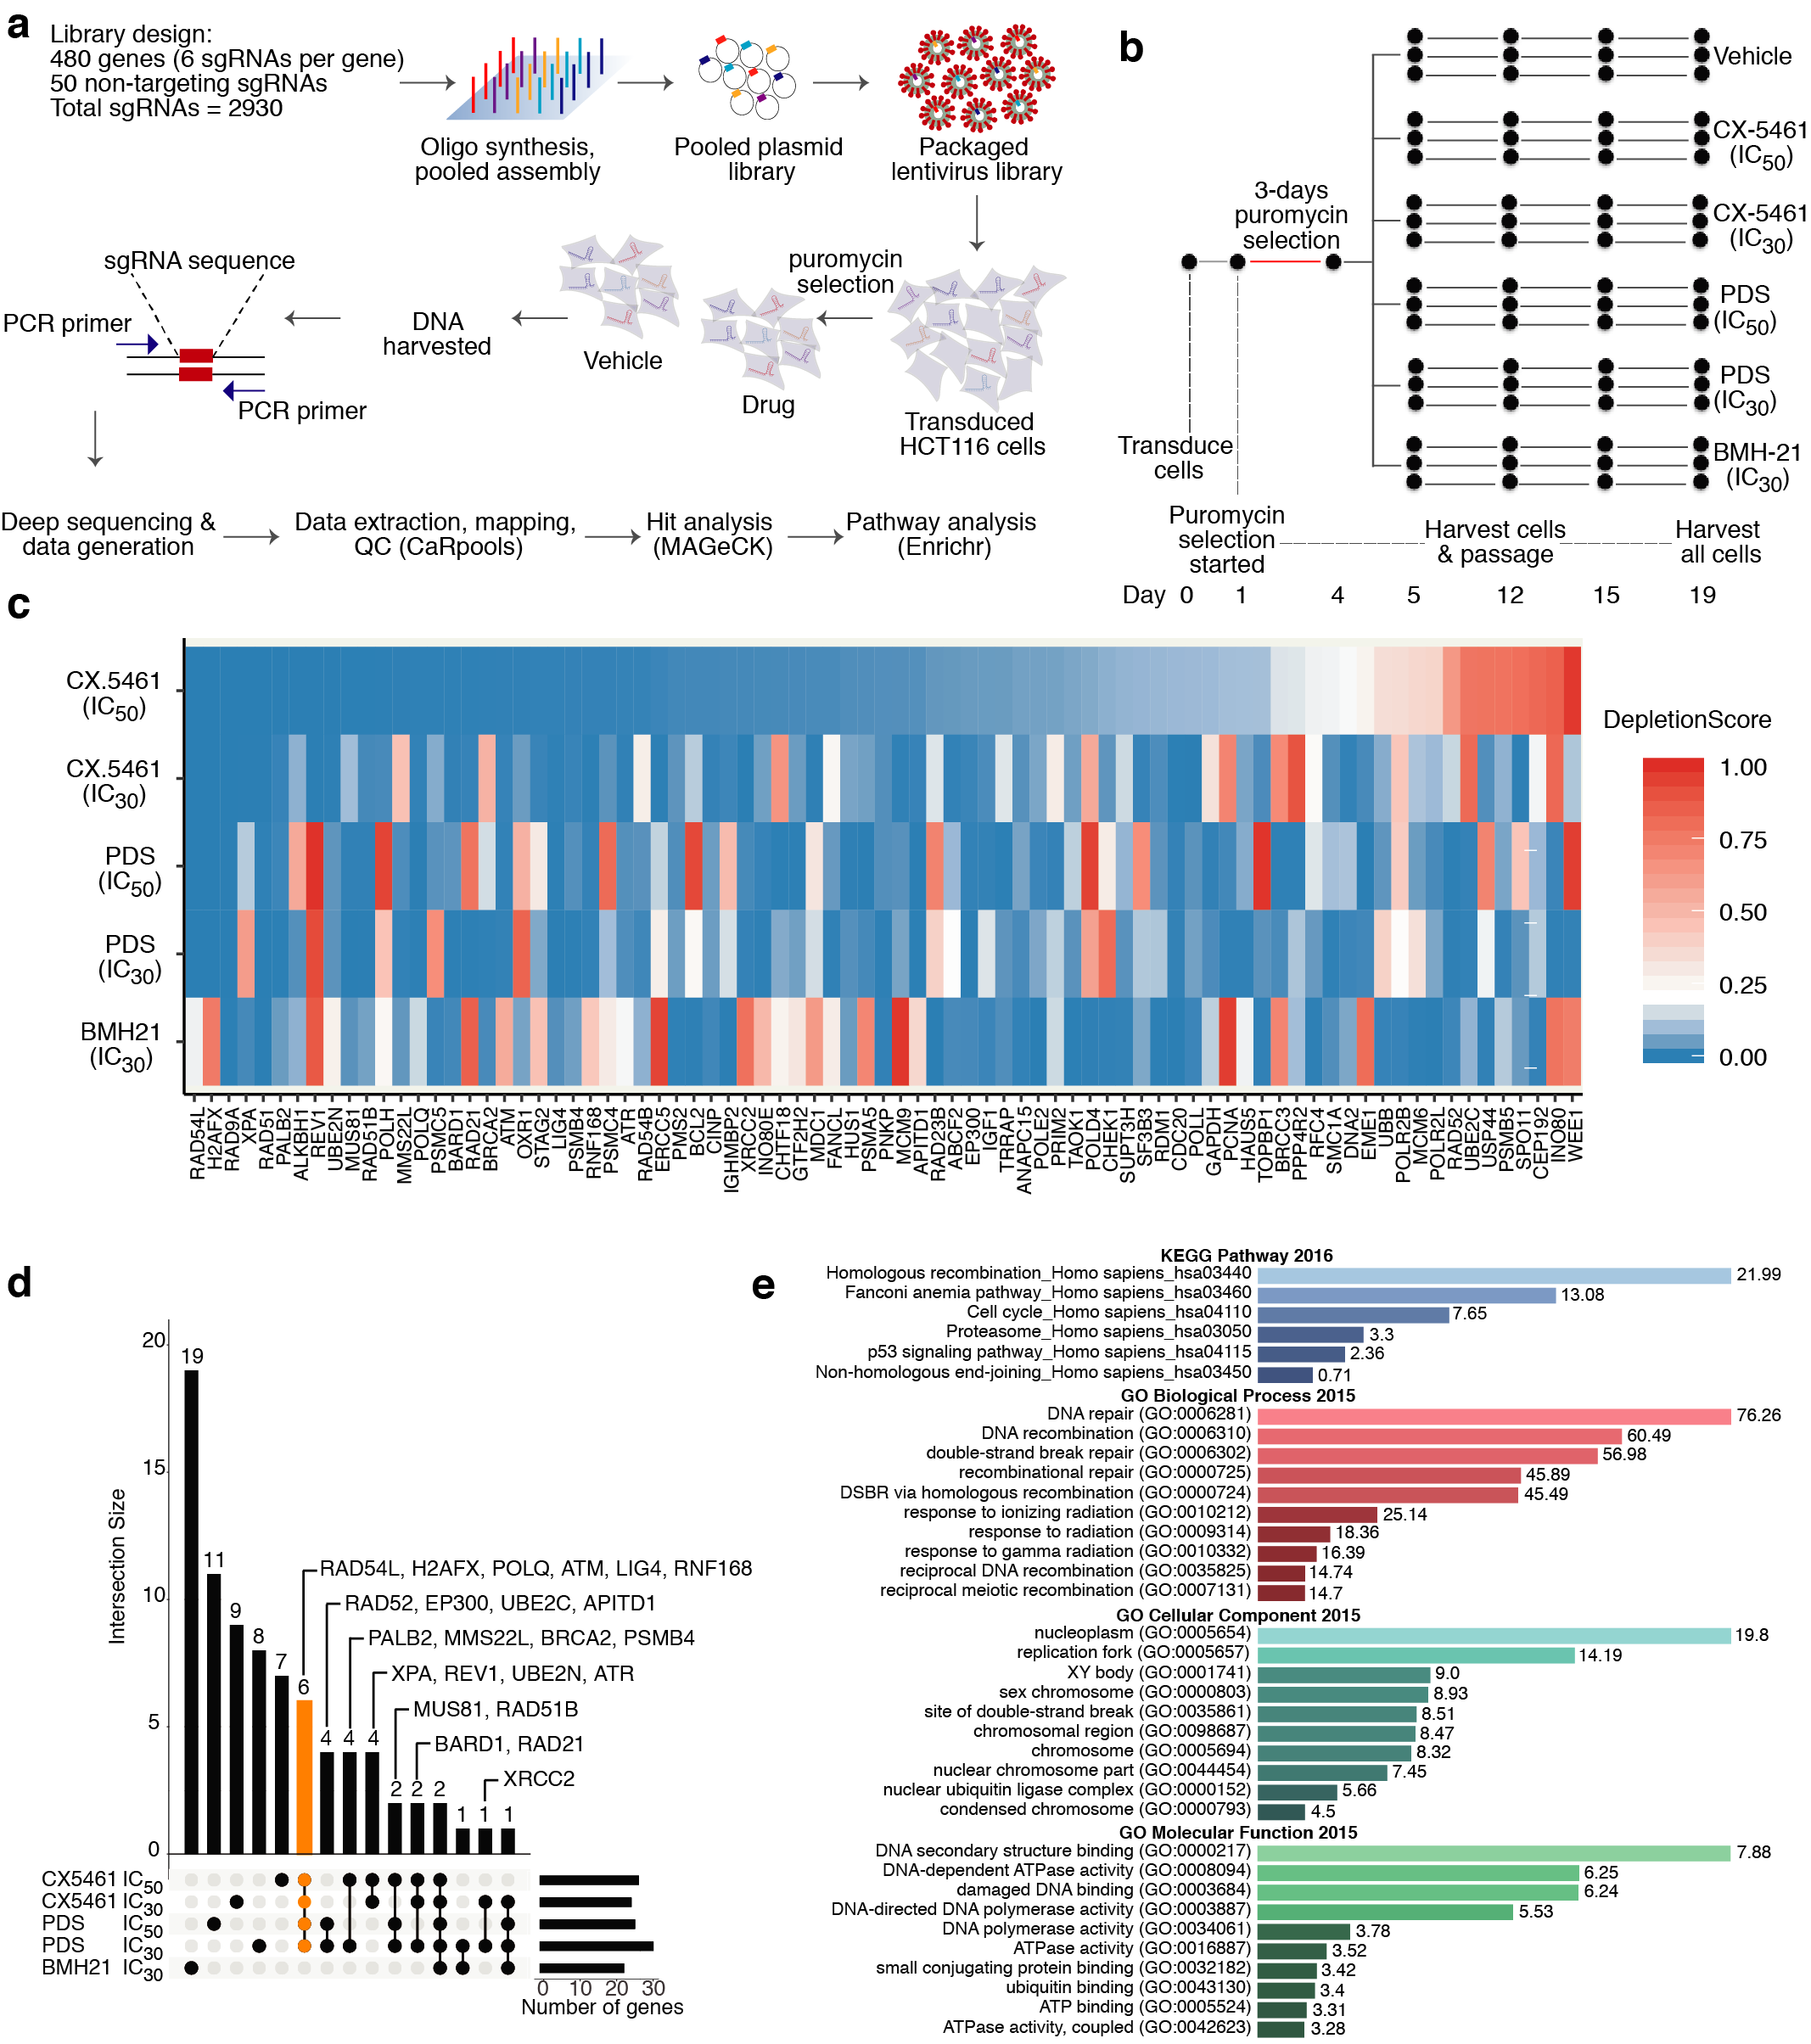
\includegraphics[width=1\textwidth]{../figures/Figure1_drug_screen}
    \caption[CX-5461 genetic screen schema]
            {\small{\textbf{Pooled CRISPR-Cas9 screens reveal genetic determinants of sensitivity to G4 drugs.}}
            }
        \label{fig:drug-screen}
\end{figure}
\addtocounter{figure}{-1}
\begin{figure}
  \caption{
        \newline
        \textbf{a}, Schematic of pooled screen.
        \newline
        \textbf{b}, Experimental design of drug screens. 
        \newline
        \textbf{c}, Top 81 depleted genes from MAGeCK output. Each row represents the corresponding drug treatment groups. Heatmap shows the MAGeCK depletion scores of the genes. The heatmap is ordered according to the depletion scores of CX-5461 (IC$_{50}$) group, ranking the most depleted genes on the left. To emphasize genes with the highest depletion score, the median of the color gradient (white) was shifted to 0.2.
        \newline
        \textbf{d}, The intersection of candidate genes undergoing negative selection with G4 stabilizers (P-value $<$ 0.045). In the bottom matrix, each row represents the corresponding drug set, and each column represents the intersection. The numbers on the right of the matrix indicate the number of genes in the input sets. The number of genes in each intersection is represented by the dynamite plot (top). Gene hits common in all CX-5461 and PDS conditions are shown in  yellow.
        \newline
        \textbf{e}, KEGG pathway and Gene Ontology enrichment analysis for 58 genes hits (P-value of $<$0.045) exclusive to CX-5461 and PDS screens was performed using Enrichr. A combined score was calculated using the P-value computed from Fisher exact test and z-score of the deviation from the expected rank. The top enriched categories are shown, ranked by the combined score (represented by the length of the bar). The brightness of the color indicates the significance. The numbers adjacent to the bars indicate the combined score.  
  }
\end{figure}
\clearpage

\begin{figure}
    \centering
    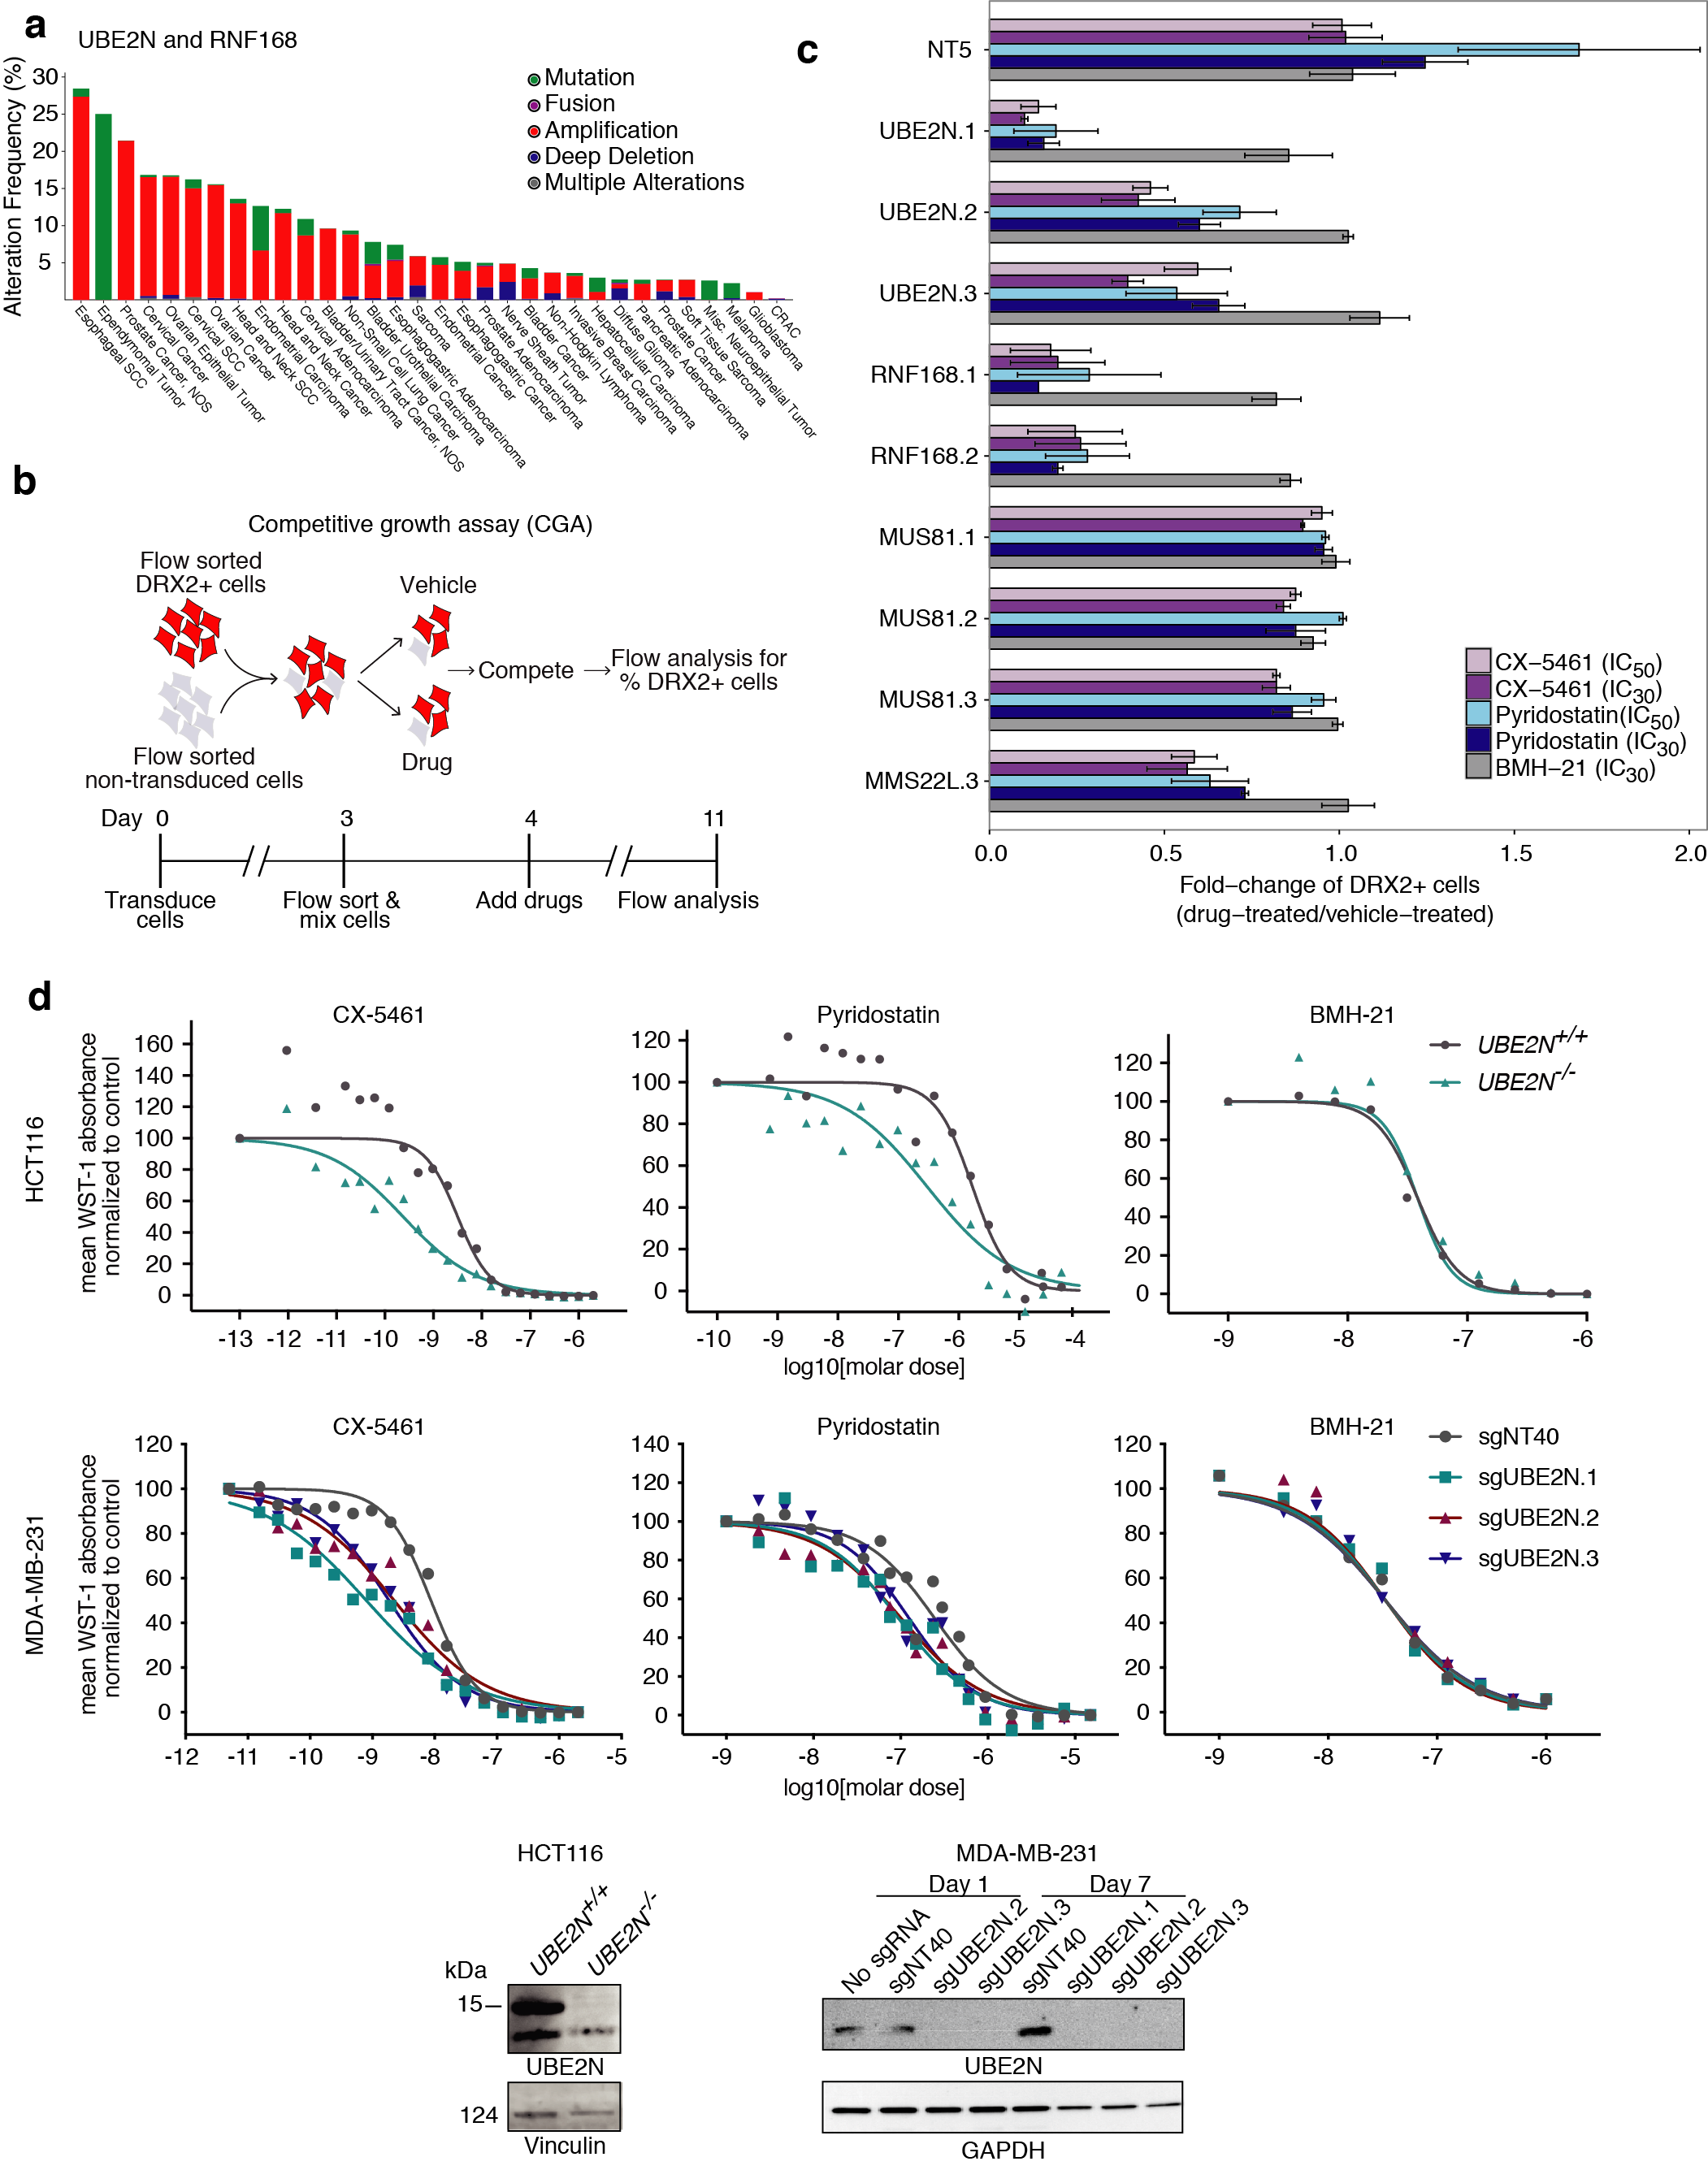
\includegraphics[width=1\textwidth]{../figures/Figure2_genetic_validation}
    \captionof{figure}[Screen validation]
            {\small{\textbf{Validation of CX-5461 and Pyridostatin drug screens in HCT116 cells.}}
            }
        \label{fig:genetic-validation}
\end{figure}

\addtocounter{figure}{-1}
\begin{figure}
  \caption{
        \newline
        \textbf{a}, Genetic alterations in UBE2N and RNF168 genes in different cancers with a minimum of 2\% of altered cases in each cancer type determined from CBioPortal database. SCC=Squamous cell carcinoma, CRAC=Colorectal Adenocarcinoma.
        \newline
        \textbf{b}, Outline of competitive growth assays (CGA).
        \newline
        \textbf{c}, HCT116 cells were transduced with individual sgRNAs including a non-targeting control (NT5), three targeting UBE2N, two for RNF168, three for MUS81, one for MMS22L. Transduced and non-transduced mixed cell populations were subjected to different drug treatments for one week at indicated doses and flow analysis was performed to determine the fraction of cells expressing red fluorescence. The mean relative fold change to vehicle treatment is shown (bar) for each mixed population with the standard error of means (SEM). The results are representative of at least two independent experiments, and three technical replicates for each experiment.
        \newline
        \textbf{d}, HCT116 UBE2N-wildtype (+/+) and -null cells (-/-) (top panel) were treated with serial dilutions of CX-5461, PDS, and BMH-21 for a week followed by WST-1 assay. The Western blot shows UBE2N gene expression in both cell lines. MDA-MB-231 cells (bottom panel) were transduced with lentivirus targeting UBE2N gene or a non-targeting control (NT40) and treated with serial dilutions of CX-5461, PDS and BMH-21 for one week followed by WST-1 assay. The Western blot shows UBE2N gene expression in all the cell lines at the start of the drug treatment (day 1) and at the end of the experiment (day 7). The results are representative of at least two independent experiments, and three technical replicates for each experiment.
        }
\end{figure}
\clearpage

\begin{figure}
    \centering
    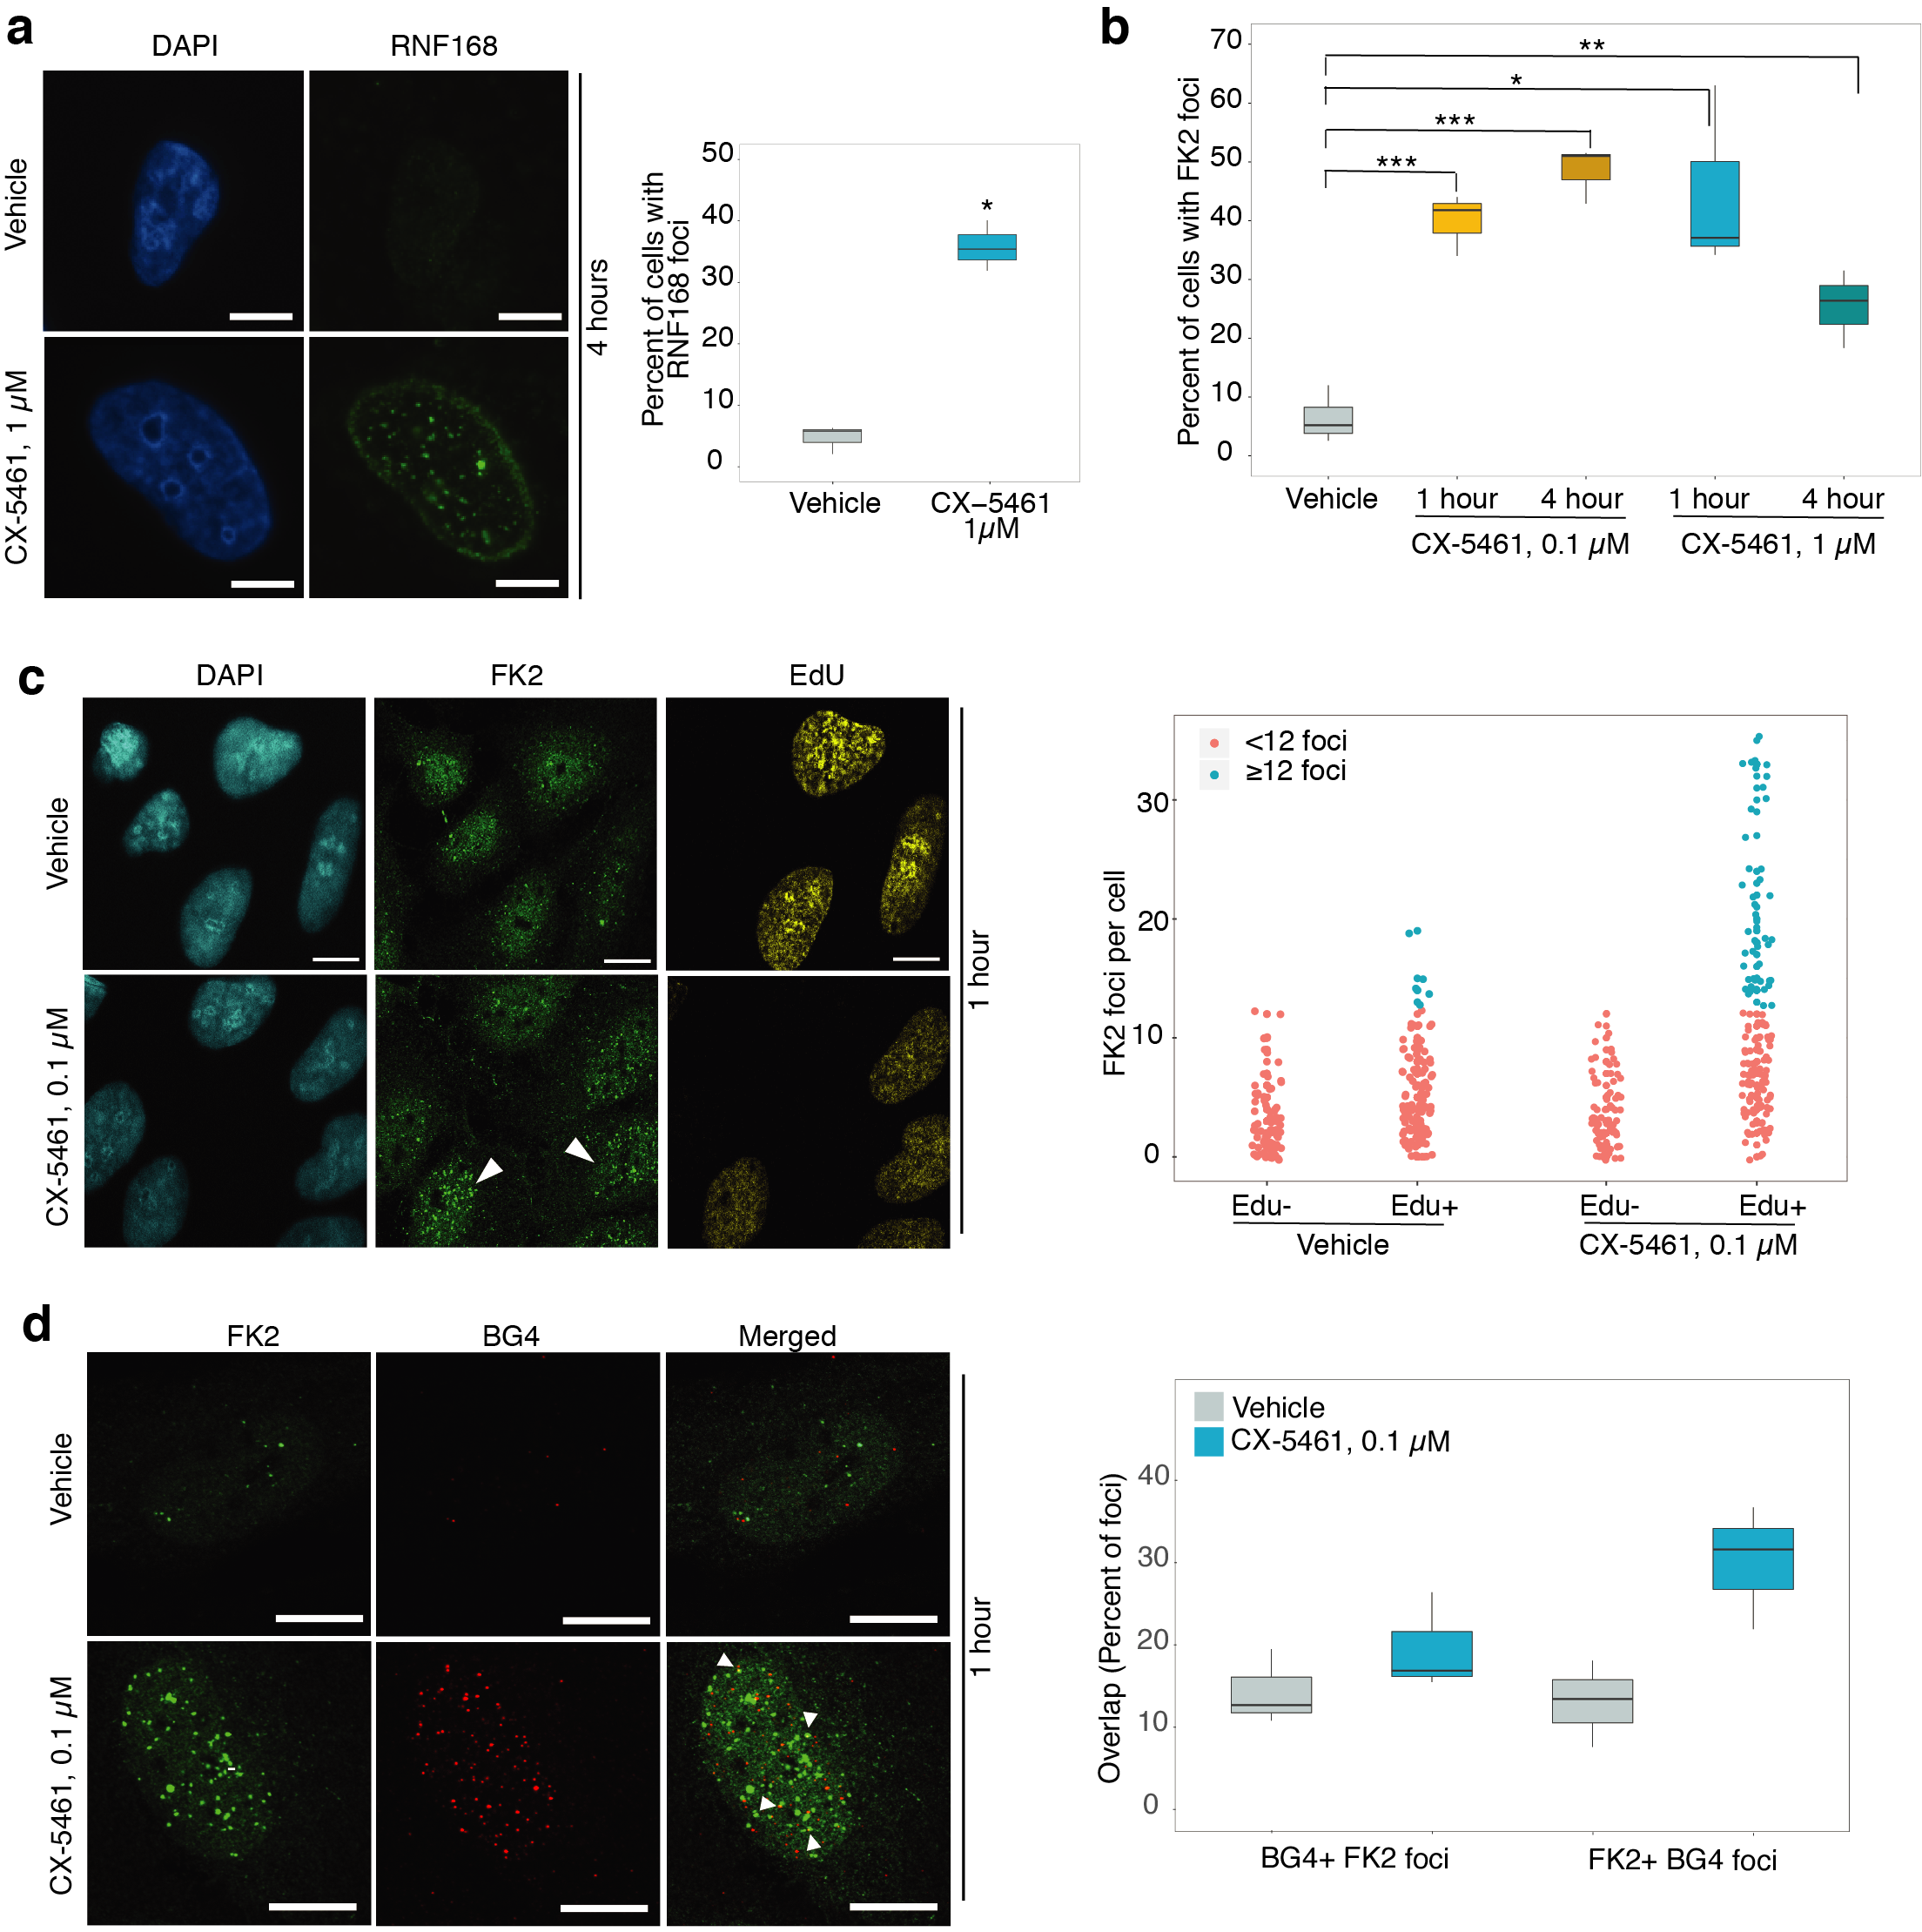
\includegraphics[width=1\textwidth]{../figures/Figure3_Ub_signaling_foci}
    \caption[CX5461 induced ubiquitin signaling]
            {\small{\textbf{DDR-associated ubiquitin signaling is activated by CX-5461 treatment.}}
            }
        \label{fig:ubiquitin-signaling}
\end{figure}
\addtocounter{figure}{-1}
\begin{figure}
  \caption[]{
        \newline
        \textbf{a}, RNF168 foci were induced in U2OS cells after 4 hours of incubation with \SI{1}{\micro\Molar} CX-5461. Left panel shows the images of RNF168 and DAPI staining. Right panel shows the percent of cells with RNF168 foci after CX-5461 and vehicle treatments. *** P-value$<$0.001, one-tailed unpaired t-test).  
        \newline
        \textbf{b}, FK2 foci were induced in U2OS cells after CX-5461 treatment at indicated doses and durations of drug treatment. *P-value $<$ 0.05 (Welch's one-tailed t-test), **P-value $<$ 0.001 (one-tailed unpaired t-test), *** P-value $<$ 0.0001 (one-tailed unpaired t-test).
        \newline
        \textbf{c}, CX-5461-induced FK2 foci are enriched in S-phase of cell cycle. U2OS cells were incubated with \SI{10}{\micro\Molar} EdU for 20 minutes to label S-phase cells followed by incubation with vehicle or \SI{0.1}{\micro\Molar} CX-5461 for 1 hour. Foci were visualized using confocal microscopy. The graph on the right shows the number of FK2 foci per cell in Edu- (negative) and Edu+ (positive) cells. Cells with 12 or more FK2 foci are shown as blue and the cells with less than 12 FK2 foci per cell as red. The difference in the number of FK2 foci in Edu+ cells is significant between CX5461 and vehicle treatments (P-value$<0$.0001, TukeyHSD test).
        \newline
        \textbf{d}, Co-localization of FK2 foci and BG4 foci in U2OS cells after 1 hour of treatment with either vehicle or CX-5461 at the indicated dose. The graph on the right shows the overlap of BG4 and FK2 foci as either percent of total FK2 foci that are also BG4+ (BG4+ FK2 foci) or percent of total BG4 foci that are also FK2+ (FK2+ BG4 foci). 
        \newline
        Scale bars in all experiments represent \SI{10}{\micro\Molar}. Results are representative of three independent experiments. In each experiment, at least 100 cells were counted.
        }
 \end{figure}
 \clearpage

\begin{figure}
    \centering
    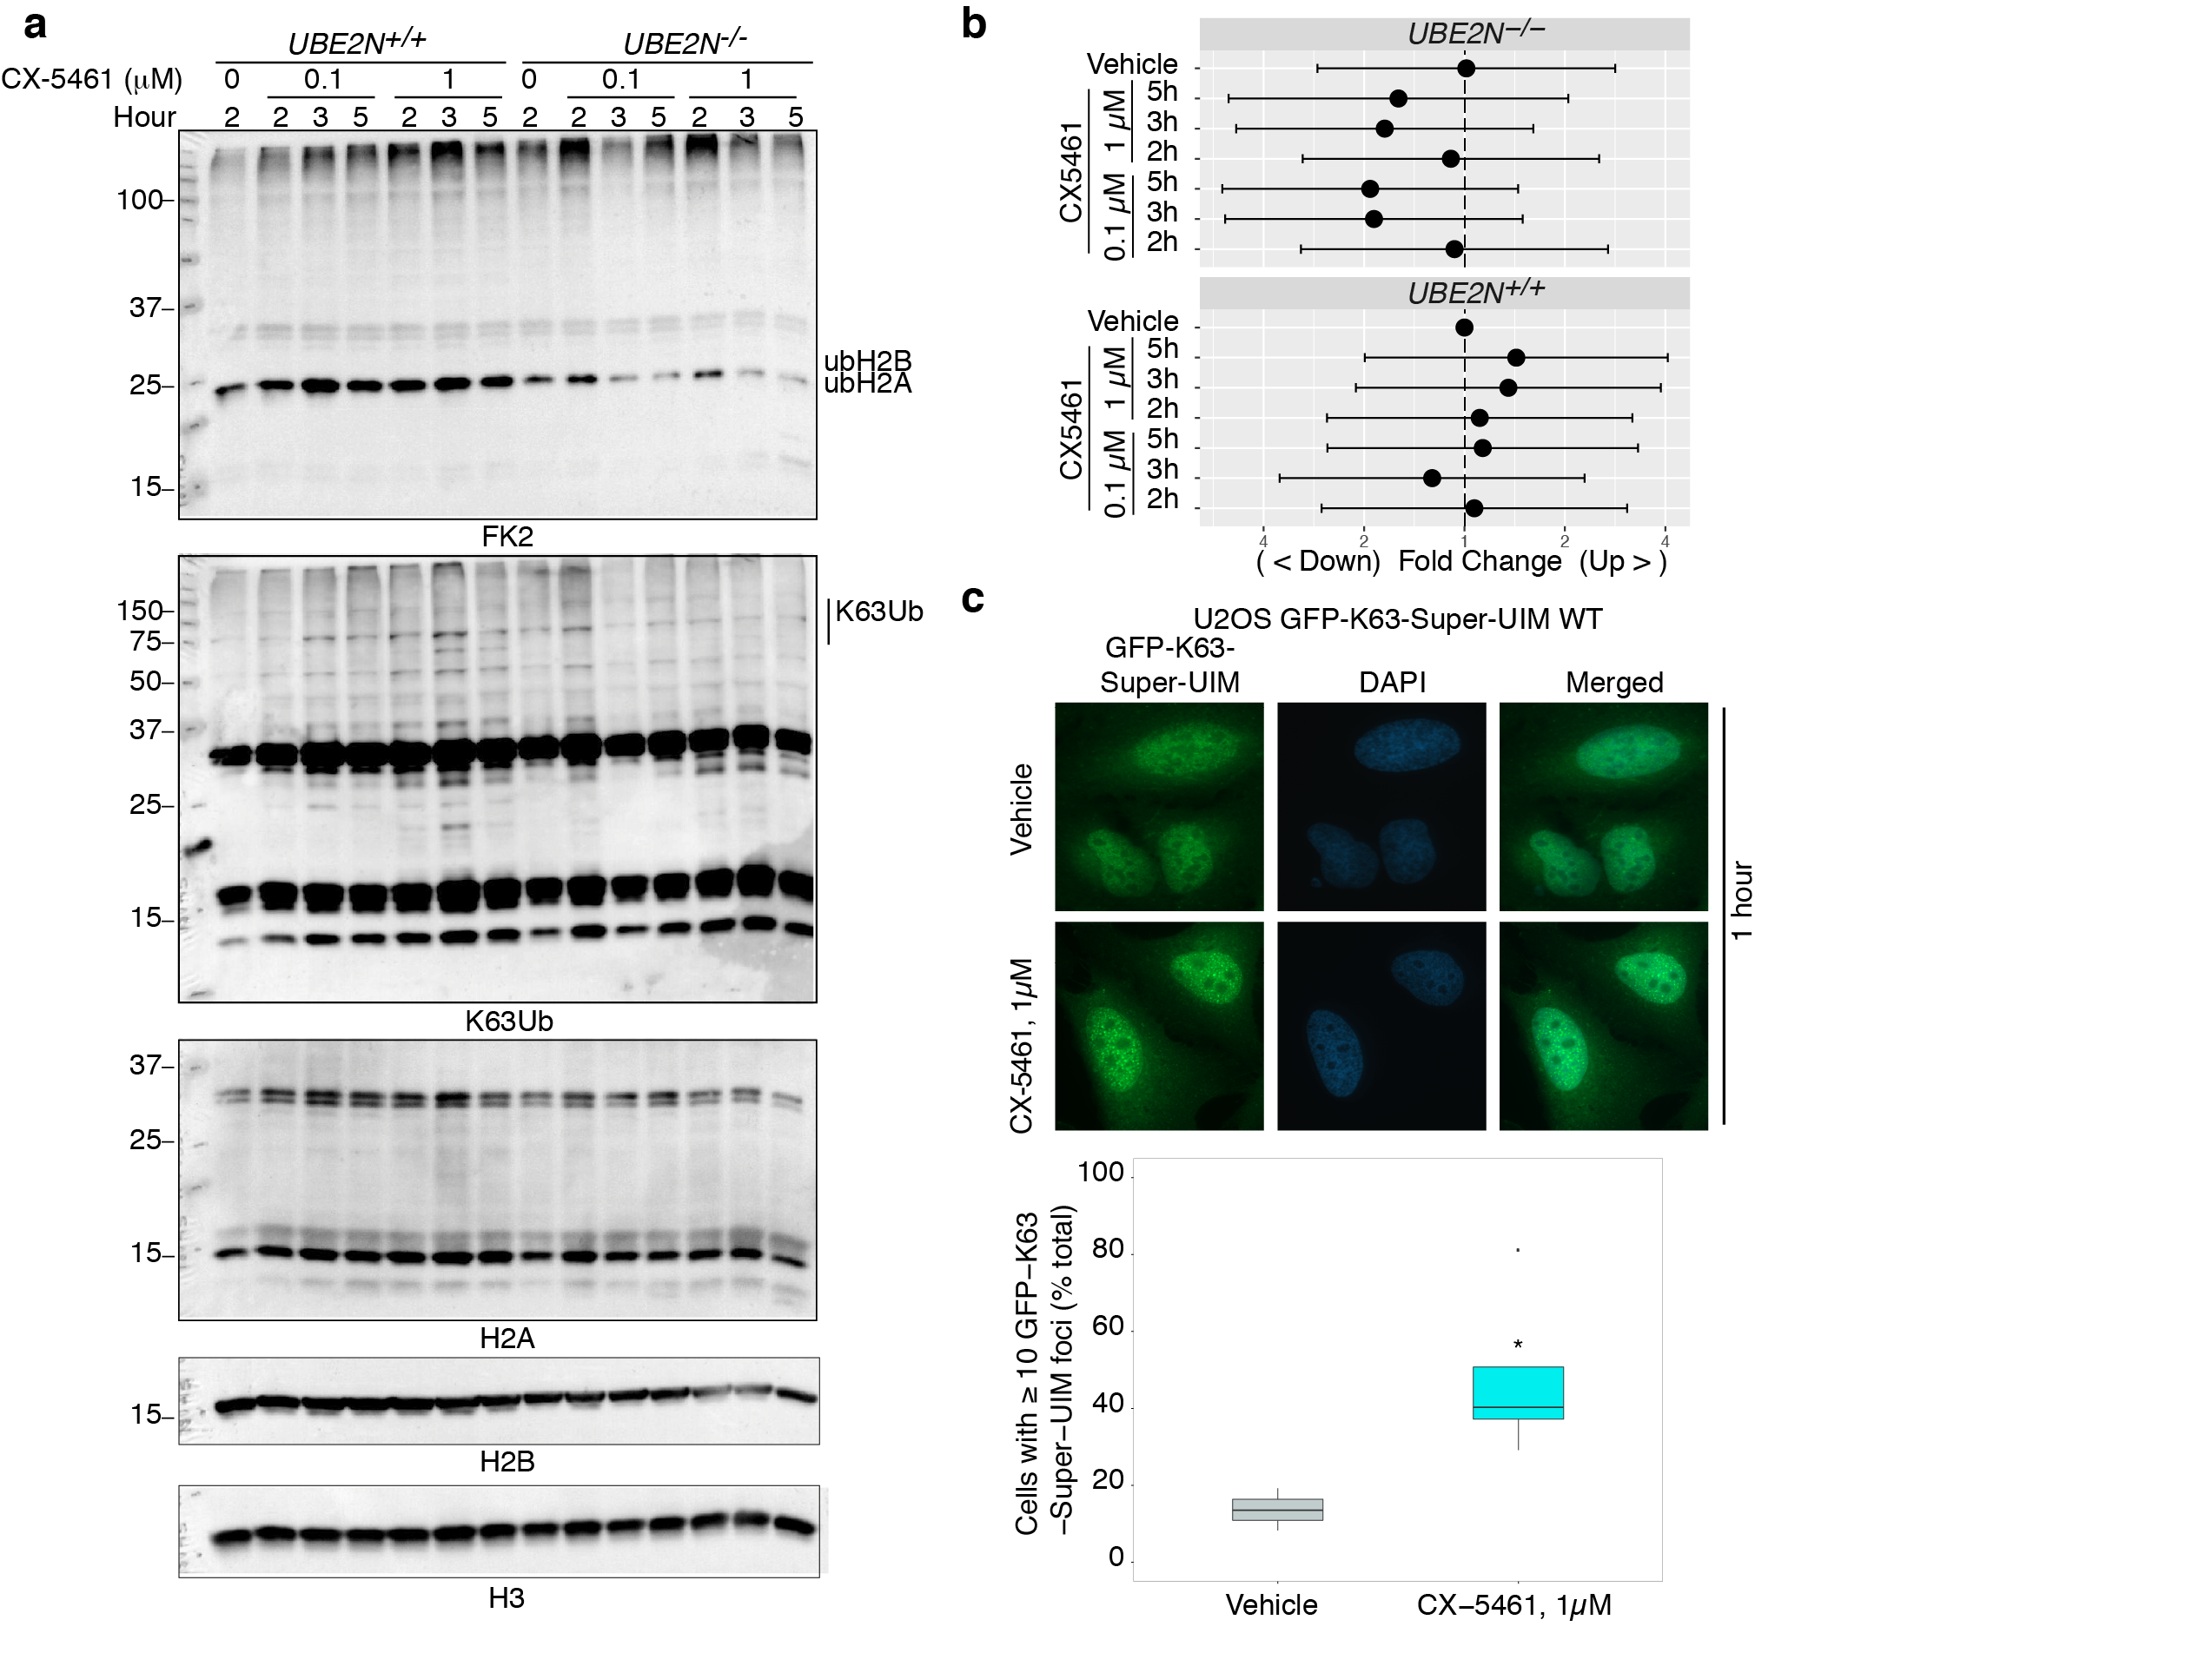
\includegraphics[width=1\textwidth]{../figures/Figure4_chromatin_ubiquitination}
    \caption[Chromatin ubiquitination]
            {\small{\textbf{CX-5461 induces K63-linked chromatin ubiquitination.}}
            }
        \label{fig:chromatin-ubiquitination}
\end{figure}
\addtocounter{figure}{-1}
\begin{figure}
  \caption[]{
        \newline
        \textbf{a}, \textit{UBE2N$^{+/+}$} and \textit{UBE2N$^{-/-}$} HCT116 cells were treated with either vehicle or CX-5461 at indicated doses and time periods, and chromatin fractions were extracted. Chromatin ubiquitination was examined using Western blots with antibodies against conjugated ubiquitin (FK2), K63-linked ubiquitin (K63Ub), histones H2A, H2B and H3. Molecular weight markers (KDa) are shown on the left. 
        \newline
        \textbf{b}, Forest plot showing UBE2N-dependent histone ubiquitination using FK2 antibody in Western blot assays described in (a). Total H2A measured via bands at 15kDa  and around 35kDa (possibly ubiquitinated H2A) provided a loading control. The dark circles indicate mean estimates of fold-change after drug treament relative to the vehicle. The horizontal bars indicate confidence interval.
        \newline
        \textbf{c}, U2OS cells with dox-inducible GFP-K63-Super-UIM were treated with either \SI{1}{\micro\Molar} CX-5461 or vehicle 24 hours after doxycycline induction. Cells were fixed at indicated time and images were obtained using the same exposure time. Cells with 10 or more foci were counted using ImageJ. For each condition, at least 100 cells were examined.  The box  plots show the median, 25\% and 75\% quantile, and outliers for the percentage of cells with ten or more foci. The results are representative of the pooled data from two independent experiments. CX-5461-treated group showed statistical significance when compared with vehicle-treated group (* P-value = 0.02832 at significance level at 0.05, one-sided unpaired t-test). 
                }
 \end{figure}
\clearpage

\begin{figure}
    \centering
    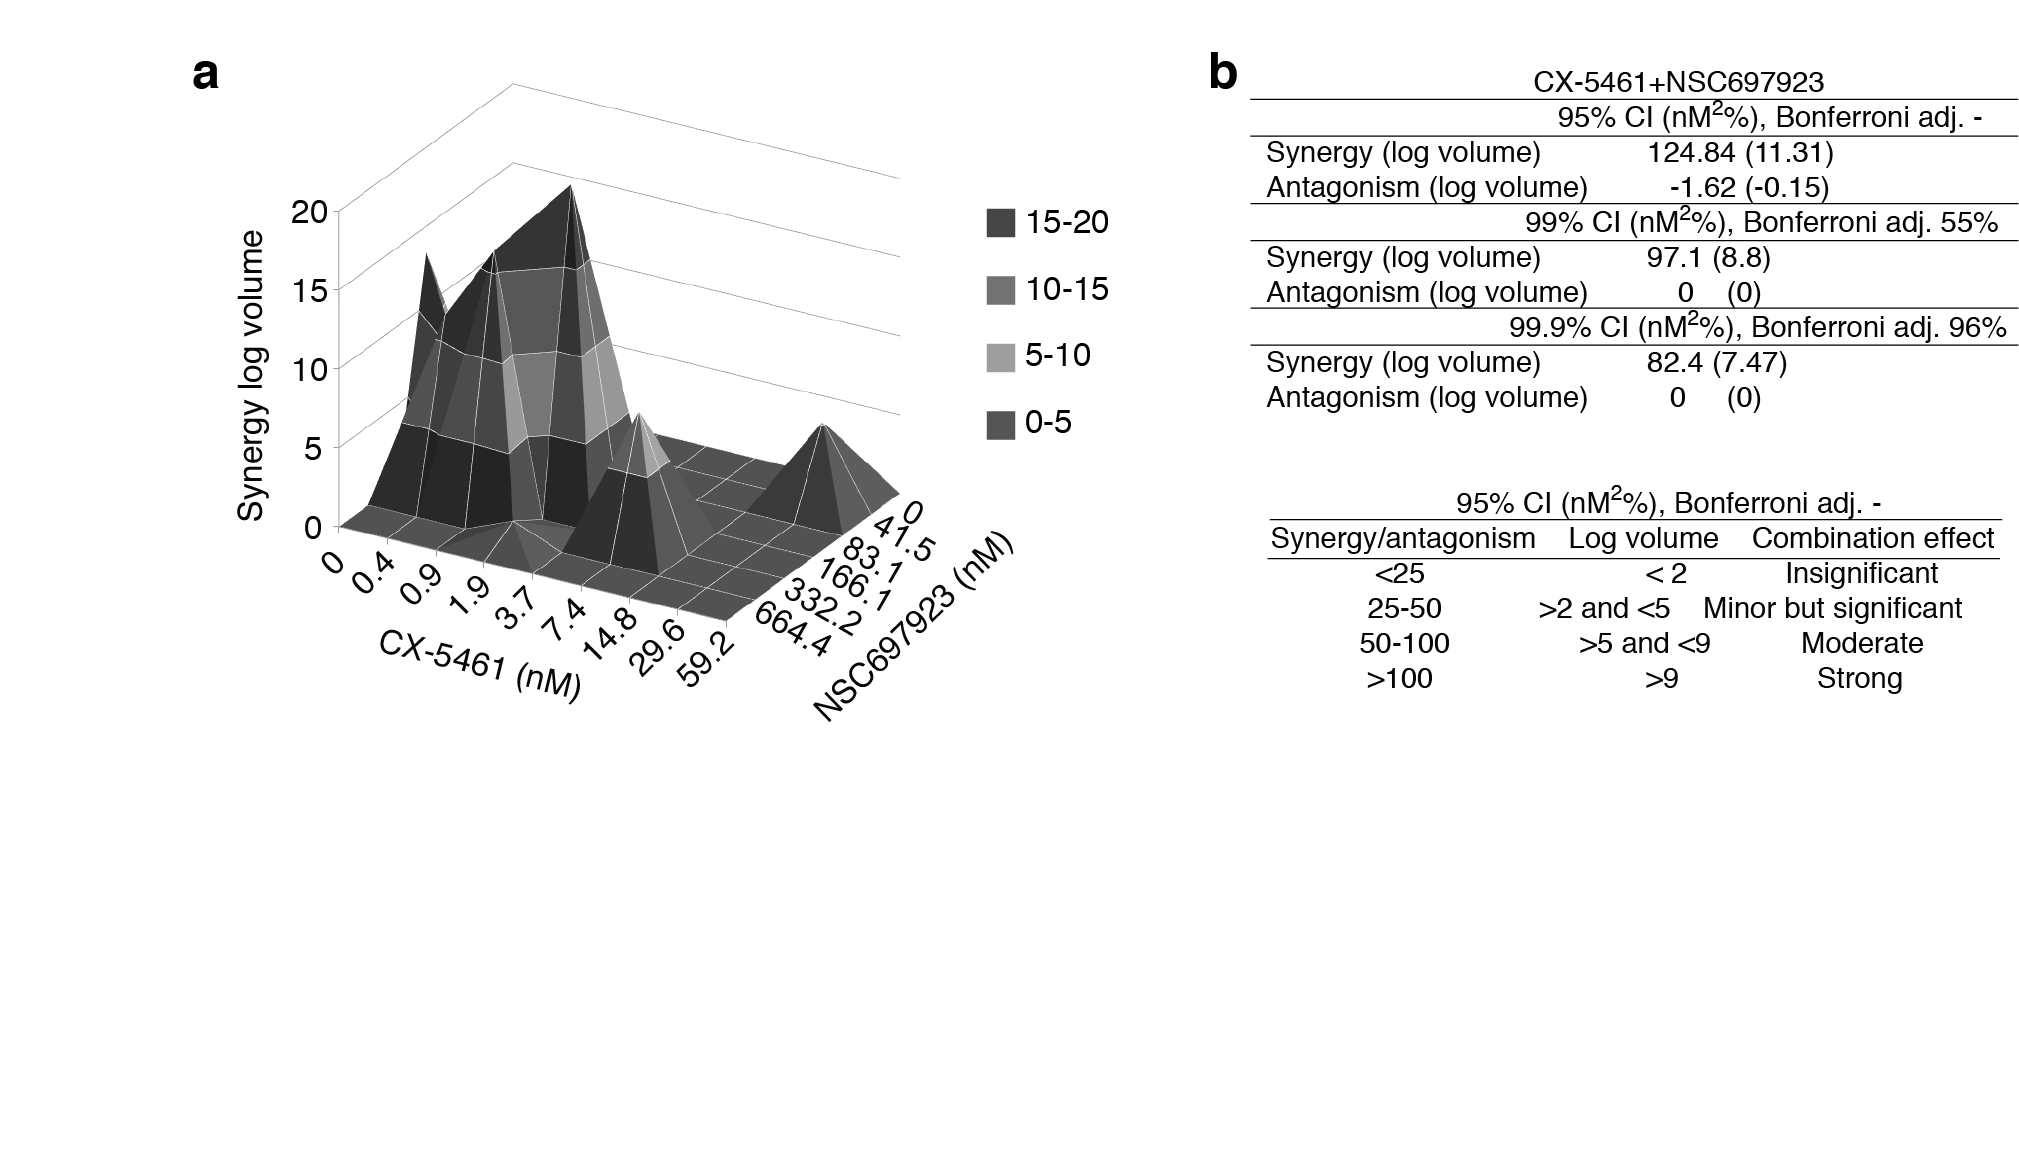
\includegraphics[width=1\textwidth]{../figures/Figure5_drug_synergy}
    \caption[Chromatin ubiquitination]
            {\small{\textbf{Pharmacological inhibition of UBE2N acts synergistically with CX-5461.}}
            \newline
            \textbf{a}, HCT116 cells were treated with serial dilutions of NSC697923 and CX-5461, as individual dilutions or as drug mixtures in 45 combinations, using equipotency ratios, for four days. NSC697923 was added at five doses and CX-5461 at nine. In the end, WST-1 assay was performed and results were analyzed to determine drug synergy using MacSynergyII software. The plot represents the volume of synergy produced by the drug combination. Cells with zero volume indicate additive interaction. A peak above zero is synergy, and depression below zero is antagonism. The index indicates the magnitude of the effect.
            \newline
            \textbf{b}, The table on the top right shows synergy or antagonism with log volumes in parentheses, at 95\%, 99\%, and 99.9\% confidence intervals (CI) calculated with the indicated Bonferroni adjustment. The table on the bottom right shows the statistically significant cut-offs for synergy and log volumes for the combination effect. The results are representative of two independent experiments with three technical replicates for each experiment.
            }
        \label{fig:drug-synergy}
\end{figure}

\clearpage

\begin{table}
\caption{Cellular Pathways Represented in the Subgenomic Library.}
\centering
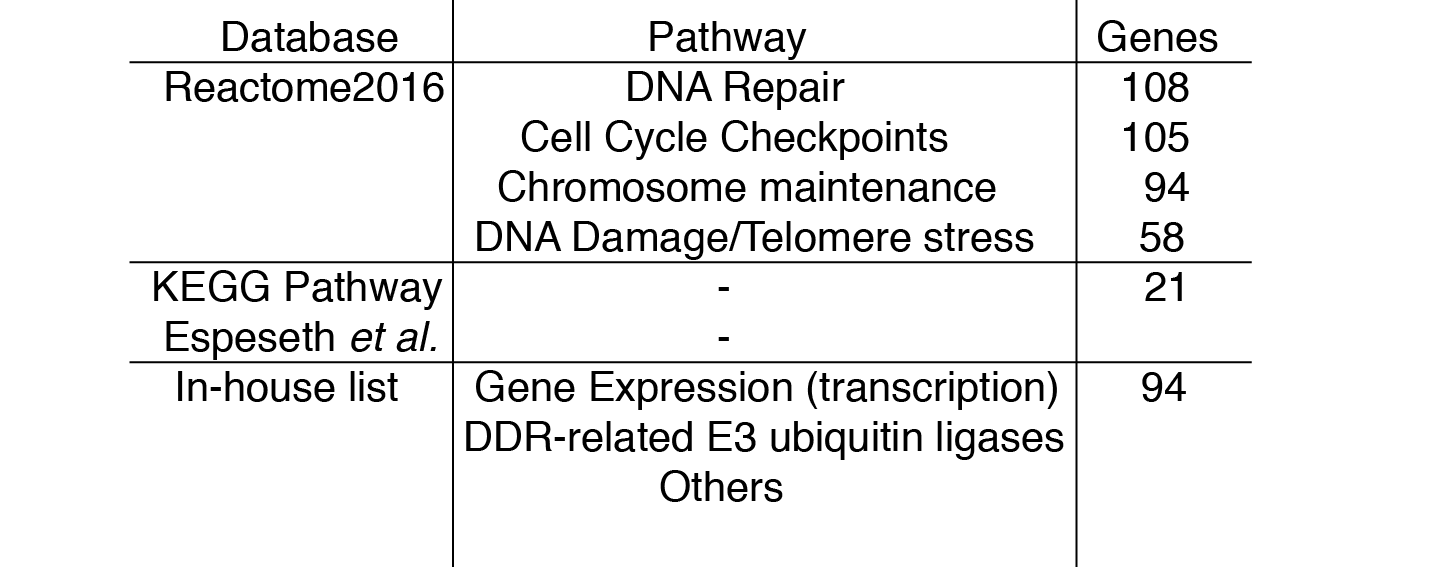
\includegraphics[width=1\textwidth]{../tables/Table1_library_design}
\label{table:library-design}
\end{table}

\clearpage

\begin{table}
\caption{Top Depleted Genes For Each Drug Treatment.}
\centering
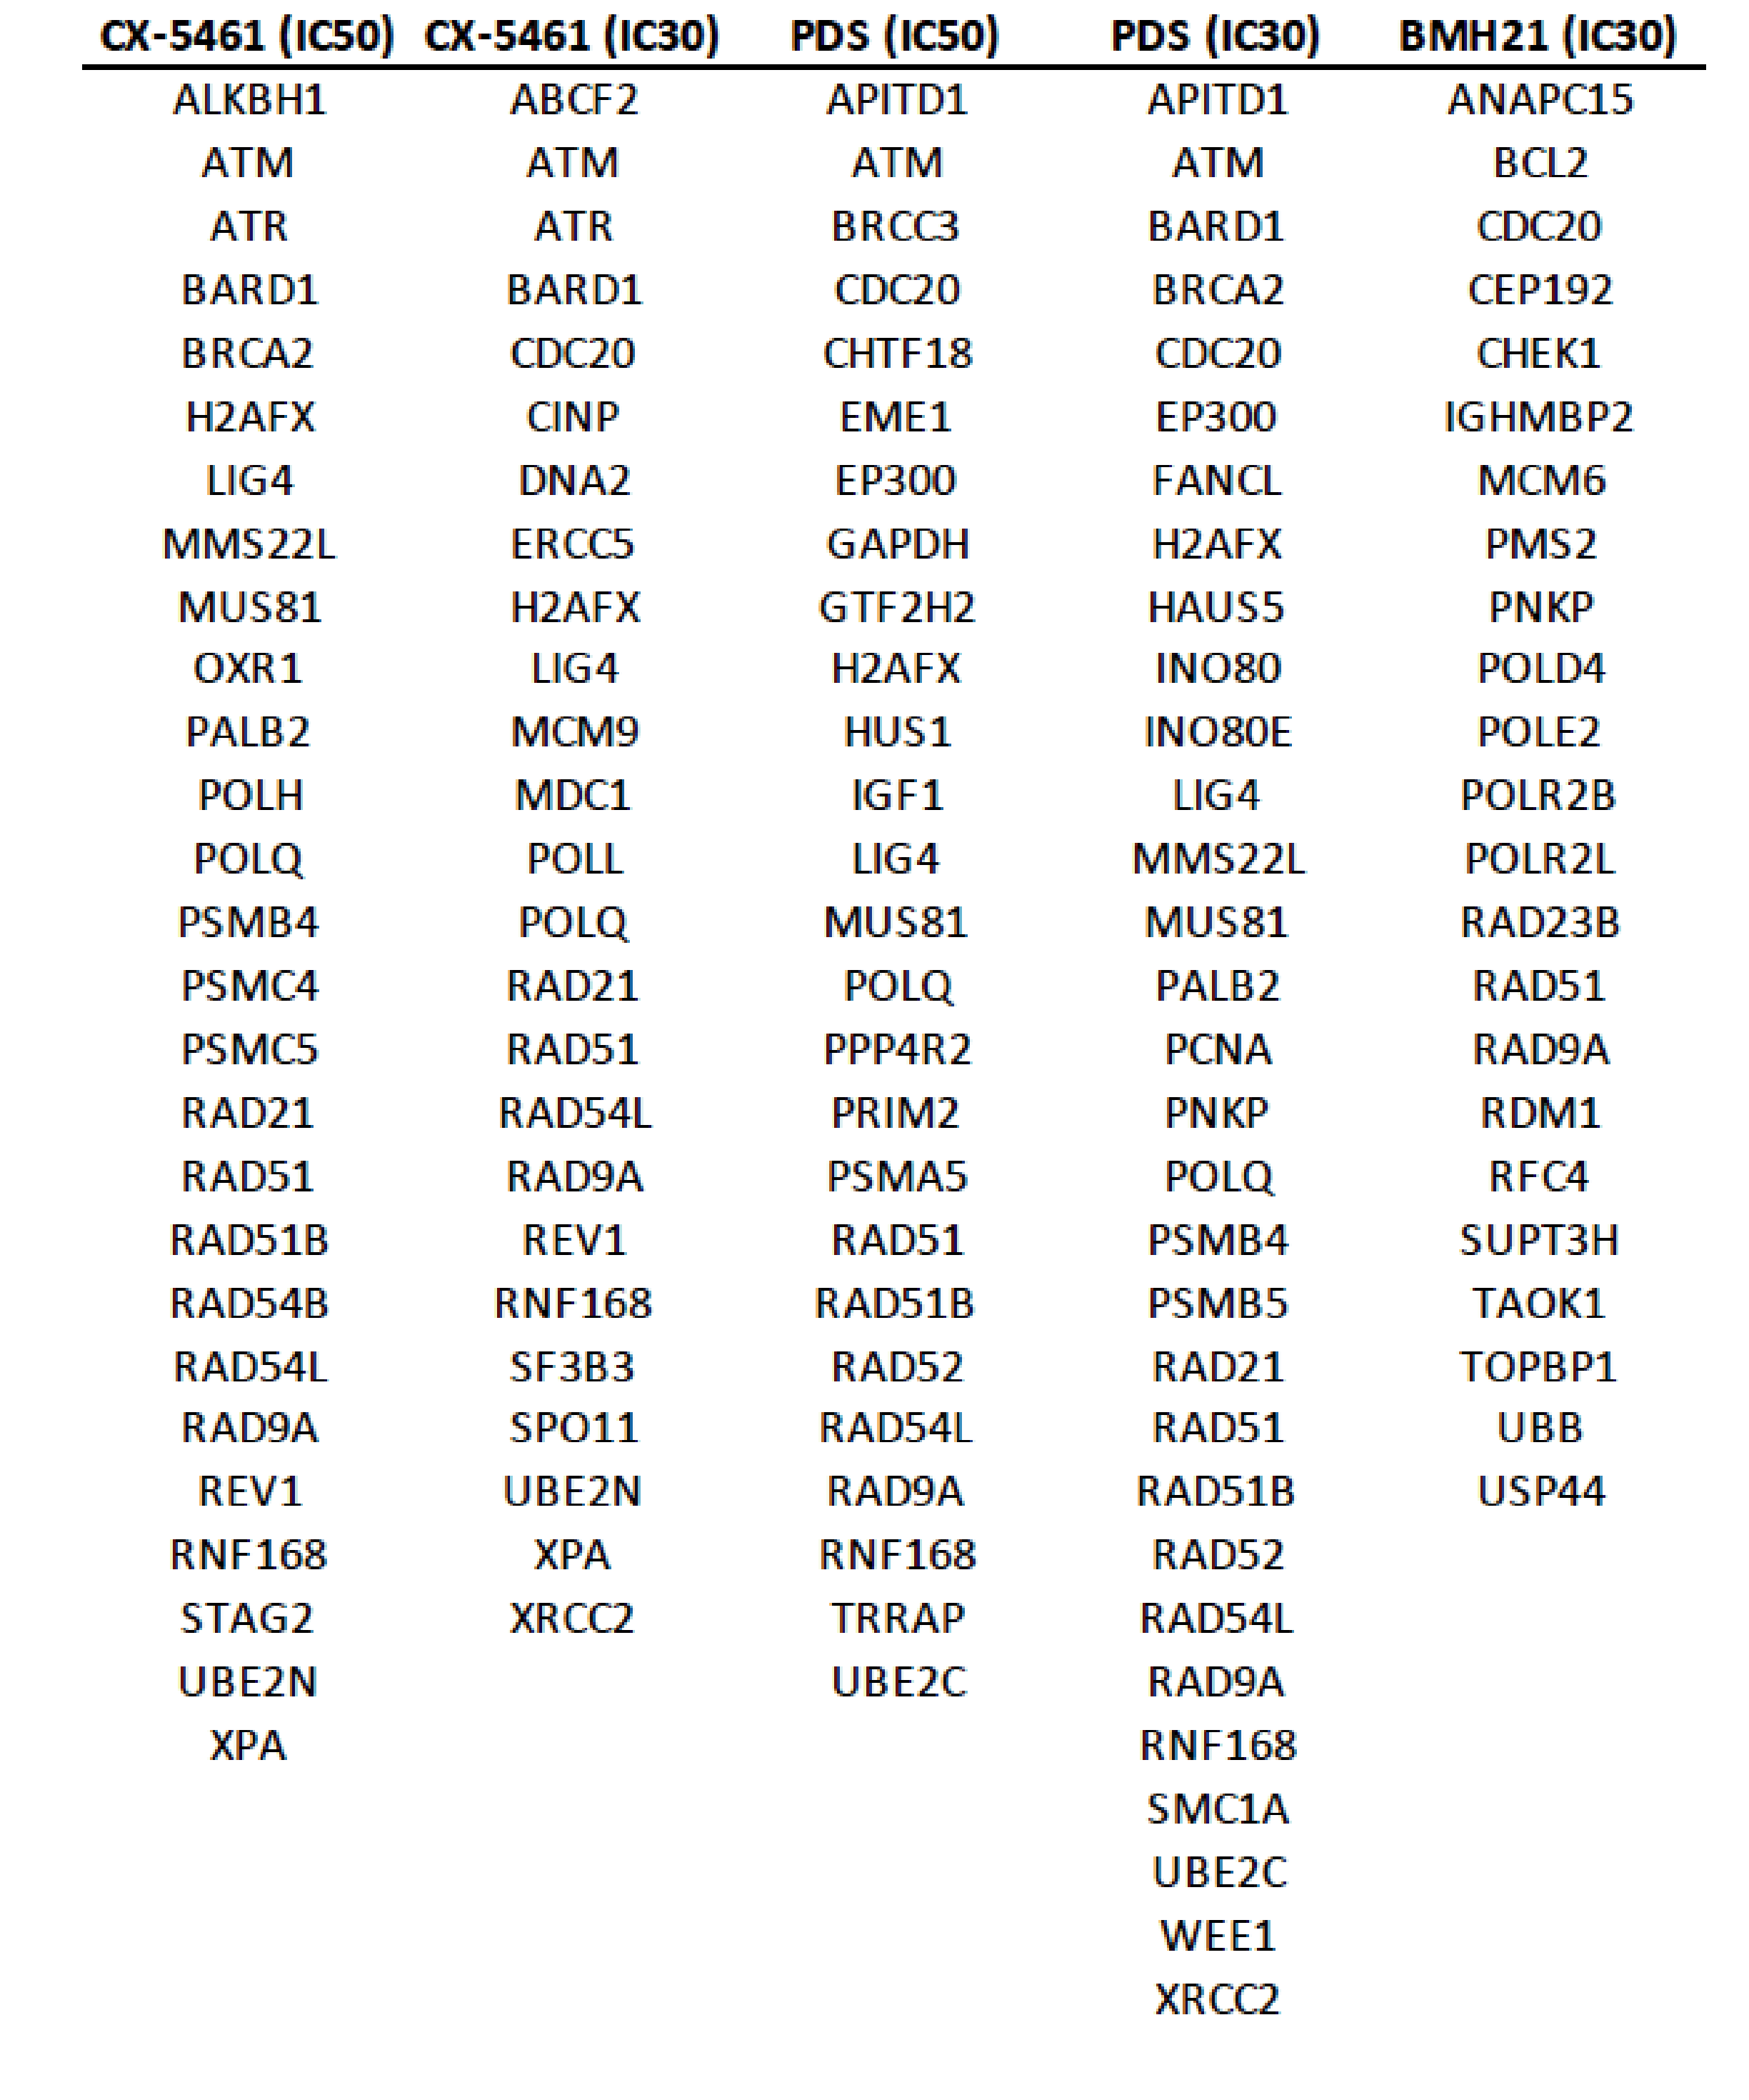
\includegraphics[width=1\textwidth]{../tables/Table1c_81_genes_list}
\label{table:81-genes list}
\end{table}

\clearpage

\begin{table}
\caption{Mean IC$_{50}$ Values, 95\% Confidence Intervals (CI) and P-values for CX-5461, Pyridostatin and BMH-21 Dose Response Upon \textit{UBE2N} Gene Targeting.}
\centering
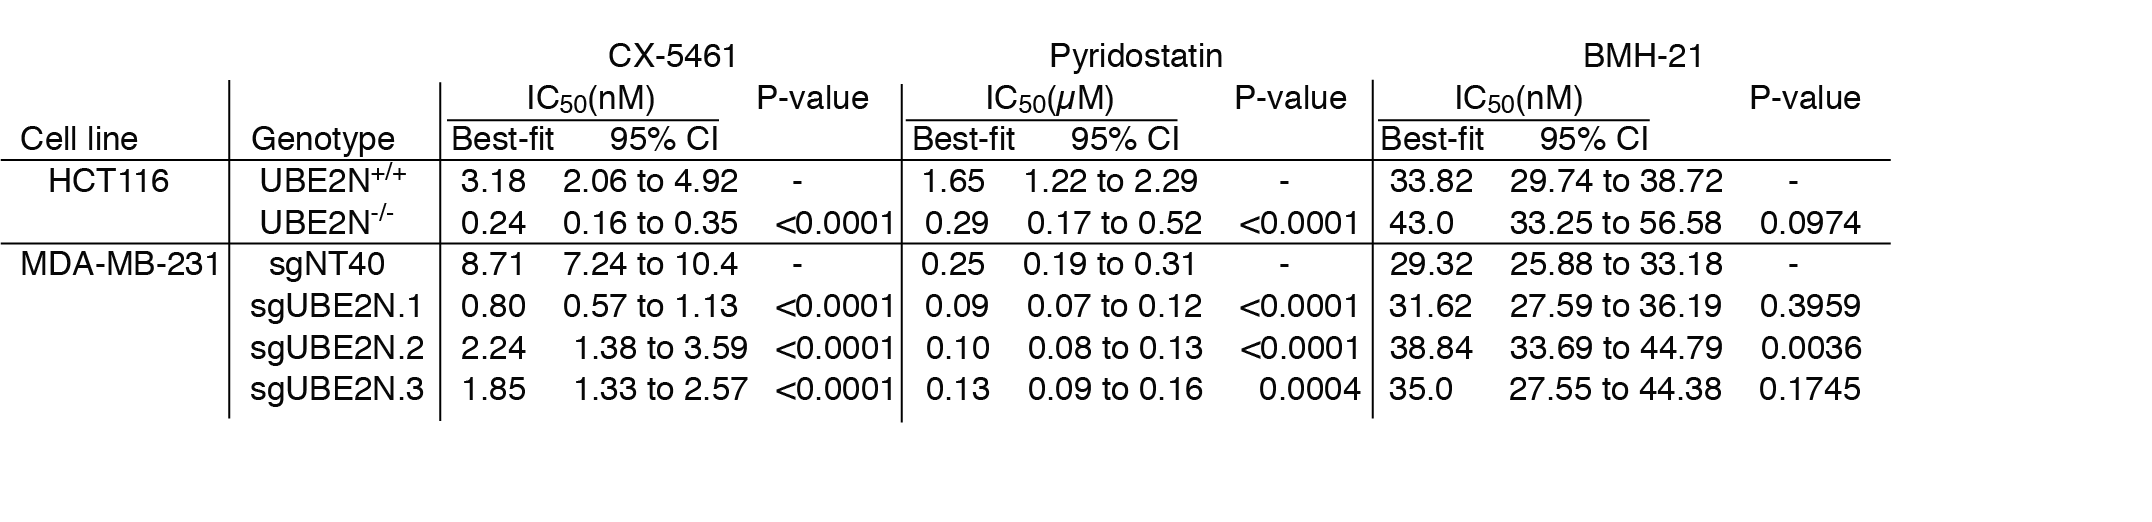
\includegraphics[width=1\textwidth]{../tables/Table_IC50}
\label{table:IC50}
\end{table}

\clearpage